%-----------------------------------------------------------------
% UNIOESTE - Centro de Engenharias e Ci�ncias Exatas
% % Modelo de relat�rio de Processamento de Imagens
% Autores: Membros do Labi e Fabiana Frata Furlan Peres
% 2011
%-----------------------------------------------------------------
%DECLARA��O DO TIPO DE DOCUMENTO, TAMANHO DA FOLHA E FONTE
%-----------------------------------------------------------------
\documentclass[normalfigtabnum,pnumromarab,normaltoc,12pt]{abnt}

%-----------------------------------------------------------------
%DEFINI��O DOS PACOTES UTILIZADOS
%-----------------------------------------------------------------
\usepackage[abnt-emphasize=bf, abnt-full-initials=yes, abnt-alf, abnt-etal-cite=3]{abnt-alf}
\usepackage[alf]{abntcite}
\usepackage[pdftex]{geometry}
\geometry{a4paper,left=3cm,right=2cm,top=3.0cm,bottom=2.0cm}
\usepackage {graphicx}
\usepackage[latin1]{inputenc} %pacote com caracteres especiais latinos, 
\usepackage[brazil]{babel} %pacote que realiza hifeniza��o e tradu��o de termos do LaTeX como Bibliography 
\usepackage[paginas=nao, ordem=alf]{tabela-simbolos}
\usepackage{algorithm}  %pacote que d� suporte � representa��o de algoritmos.
\usepackage{algorithmic}
\usepackage[listofformat=subparens]{subfig}
\usepackage{multirow}

\usepackage{graphicx,color}

%-----------------------------------------------------------------
%TERMOS RENOMEADOS
%-----------------------------------------------------------------
\floatname{algorithm}{Algoritmo} %Renomeia o termo Algorithm para Algoritmo, em uma legenda de algoritmo
\renewcommand{\listalgorithmname}{Lista de Algoritmos} %renomeia o nome da lista de algoritmos, 
\renewcommand{\listofabreviationsname}{Lista de Abreviaturas}
\renewcommand{\arraystretch}{1.5}
\newtheorem{defi}{{\bf Defini��o}}
%-----------------------------------------------------------------

%--------------------------------------------------------------
%DEFINI��O DE FORMATA��ES
%--------------------------------------------------------------
\providecommand{\Jinstituicao}{}
\renewcommand{\instituicao}[1]{\renewcommand{\Jinstituicao}{#1}}
\renewcommand{\instituicaoformat}{\scshape}

\providecommand{\Jtitulo}{}
\renewcommand{\titulo}[1]{\renewcommand{\Jtitulo}{#1}}
\renewcommand{\tituloformat}{\normalsize\ABNTchapterfont}

\providecommand{\Jlocal}{}
\renewcommand{\local}[1]{\renewcommand{\Jlocal}{#1}}
\renewcommand{\localformat}{\normalsize}

\providecommand{\Jdata}{}
\renewcommand{\data}[1]{\renewcommand{\Jdata}{#1}}
\renewcommand{\dataformat}{\normalsize}

\providecommand{\Jautor}{}
\renewcommand{\autor}[1]{\renewcommand{\Jautor}{#1}}
\renewcommand{\autorformat}{\normalsize\ABNTsectionfont}

\providecommand{\Jcomentario}{}
\renewcommand{\comentario}[1]{\renewcommand{\Jcomentario}{#1}}
\renewcommand{\comentarioformat}{}

\providecommand{\Jorientador}{}
\providecommand{\Jorientadorname}{}
\renewcommand{\orientador}[2][Orientador:\vspace{1mm}\\]{\renewcommand{\Jorientadorname}{#1} \renewcommand{\Jorientador}{#2}}
\renewcommand{\orientadornameformat}{}
\renewcommand{\orientadorformat}{\normalsize}

\providecommand{\Jcoorientador}{}
\providecommand{\Jcoorientadorname}{}
\renewcommand{\coorientador}[2][Co-orientador:\vspace{1mm}\\] {\renewcommand{\Jcoorientadorname}{#1} \renewcommand{\Jcoorientador}{#2}}
\renewcommand{\coorientadornameformat}{}
\renewcommand{\coorientadorformat}{\normalsize}

%-----------------------------------------------------------------
%DEFINI�AO DOS DADOS PARA CAPA E FOLHA DE ROSTO
%-----------------------------------------------------------------
\instituicao{UNIOESTE - UNIVERSIDADE ESTADUAL DO OESTE DO PARAN�\par
CAMPUS DE FOZ DO IGUA�U\par
CENTRO DE ENGENHARIAS E CI�NCIAS EXATAS\par
CIENCIA DA COMPUTA��O - PROCESSAMENTO DE IMAGENS}
\titulo{SDA - Sistema Distribu�do de Arquivos}
\autor{Deivide Vian\\
		Lucas Mauricio Comin}
\local{FOZ DO IGUA�U}
\data{2011}

%--------------------------------------------------------------
%CAPA
%--------------------------------------------------------------
\newcommand{\minhacapa}{
\thispagestyle{empty}
\setcounter{page}{0}
\vspace*{0cm}


\ABNTifnotempty{\Jinstituicao}
	{
		\begin{center}
			\textbf{\Jinstituicao}
	 	\end{center} 
	 }
	 
\vfill
\vfill

\ABNTifnotempty{\Jtitulo}
	{
		\begin{center}
			{\textbf{\Jtitulo}\par}
		\end{center}
	}

\vspace*{1cm}
\vfill

\ABNTifnotempty{\Jtitulo}
	{	
		\begin{center}
			{\textbf{\Jautor}}
   		\end{center}
  }
  
\vfill
\vfill

\begin{center}
  \begin{espacosimples}
    \setlength{\parskip}{.3cm}
    \ABNTifnotempty{\Jlocal}
      {\textbf{{\localformat\Jlocal}}\\ }
    \ABNTifnotempty{\Jdata}
      {\textbf{{\dataformat\Jdata}}}
  \end{espacosimples}
\end{center}


\vspace*{0cm}
\if@restonecol\twocolumn \else \newpage \fi
\espaco{\ABNTespacodefault}
}





\begin{document}

%-----------------------------------------------------------------
%CAPA, FOLHA DE ROSTO, AGRADECIMENTOS, DEDICATORIA.....
%-----------------------------------------------------------------
\minhacapa
\begin{espacoumemeio}


%-----------------------------------------------------------------
%INDICES DE FIGURAS, TABELAS, SIGLAS E CAPITULOS 
%-----------------------------------------------------------------
\clearpage
\listoffigures
%\clearpage
%\listoftables
%\clearpage
%\listadesiglas 
\clearpage 
\tableofcontents
\clearpage

%-----------------------------------------------------------------
%CAPITULOS 
%-----------------------------------------------------------------

\chapter{Descri��o do Sistema}

	\indent O objetivo do SDA � ser uma ferramenta distribu�da a qual gerencia dowload e upload de arquivos entre clientes e servidor. 
	
	O SDA possui dois m�dulos principais SDA Cliente e SDA Servidor, estes ser�o detalhados nas seguintes se��es.
	
\section{M�dulos}
		
		Os clientes do SDA que podem acessar as funcionalidades do computador SDA. Respons�vel por gerenciar as requisi��es de funcionalidades do sistema tendo a intera��o com o usu�rio atr�ves de uma interface.
		Os servi�os a serem acessados pelo SDA cliente s�o:
		
		\begin{itemize}
			\item Login: O cliente pode fazer seu login e ser autenticado no servidor;
			\item Listar todos Arquivos: Listar todos os arquivos presentes no servidor;
			\item Gravar Arquivos: Gravar Arquivos no reposit�rio do servidor;
			\item Baixar Arquivos: Gravar Arquivos no reposit�rio do pr�prio cliente;
			
		\end{itemize}
		
		J� o servidor � repons�vel pelo gerenciamento do sistema, executando as requisi��es feitas pelo m�dulo do Cliente e comunicando-se com os reposit�rios.
		
		Atividades a serem gerenciadas pelo servidor:
		
		\begin{itemize}
			\item Autenticar Clientes: Verificar autenticidade de usu�rios conectados atrav�s de dados fornecidos por estes clientes;
			\item Permitir a visualiza��o da listagem de todos arquivos;
			\item Gerenciar uploads e downloads;
		\end{itemize}
		
		As opera��es de inclus�o, exclus�o e consulta de usu�rios, est�o implementadas atrav�s RMI (Remote Method Invocation) e disp�em de algoritmos de criptografia para os dados que trafegam pela rede.
		
	As demais opera��es do sistema utilizam comunica��o UDP ou TCP quando necessitas trafegar entre canais de comunica��o.
	
\section{Diagrama de Classes do SDA}

	\indent O Diagrama de Classes do aplicativo SDA � demostrado na figura a seguir (Figura \ref{figura5}):
	
	\begin{figure}[!htb]
		\centering
		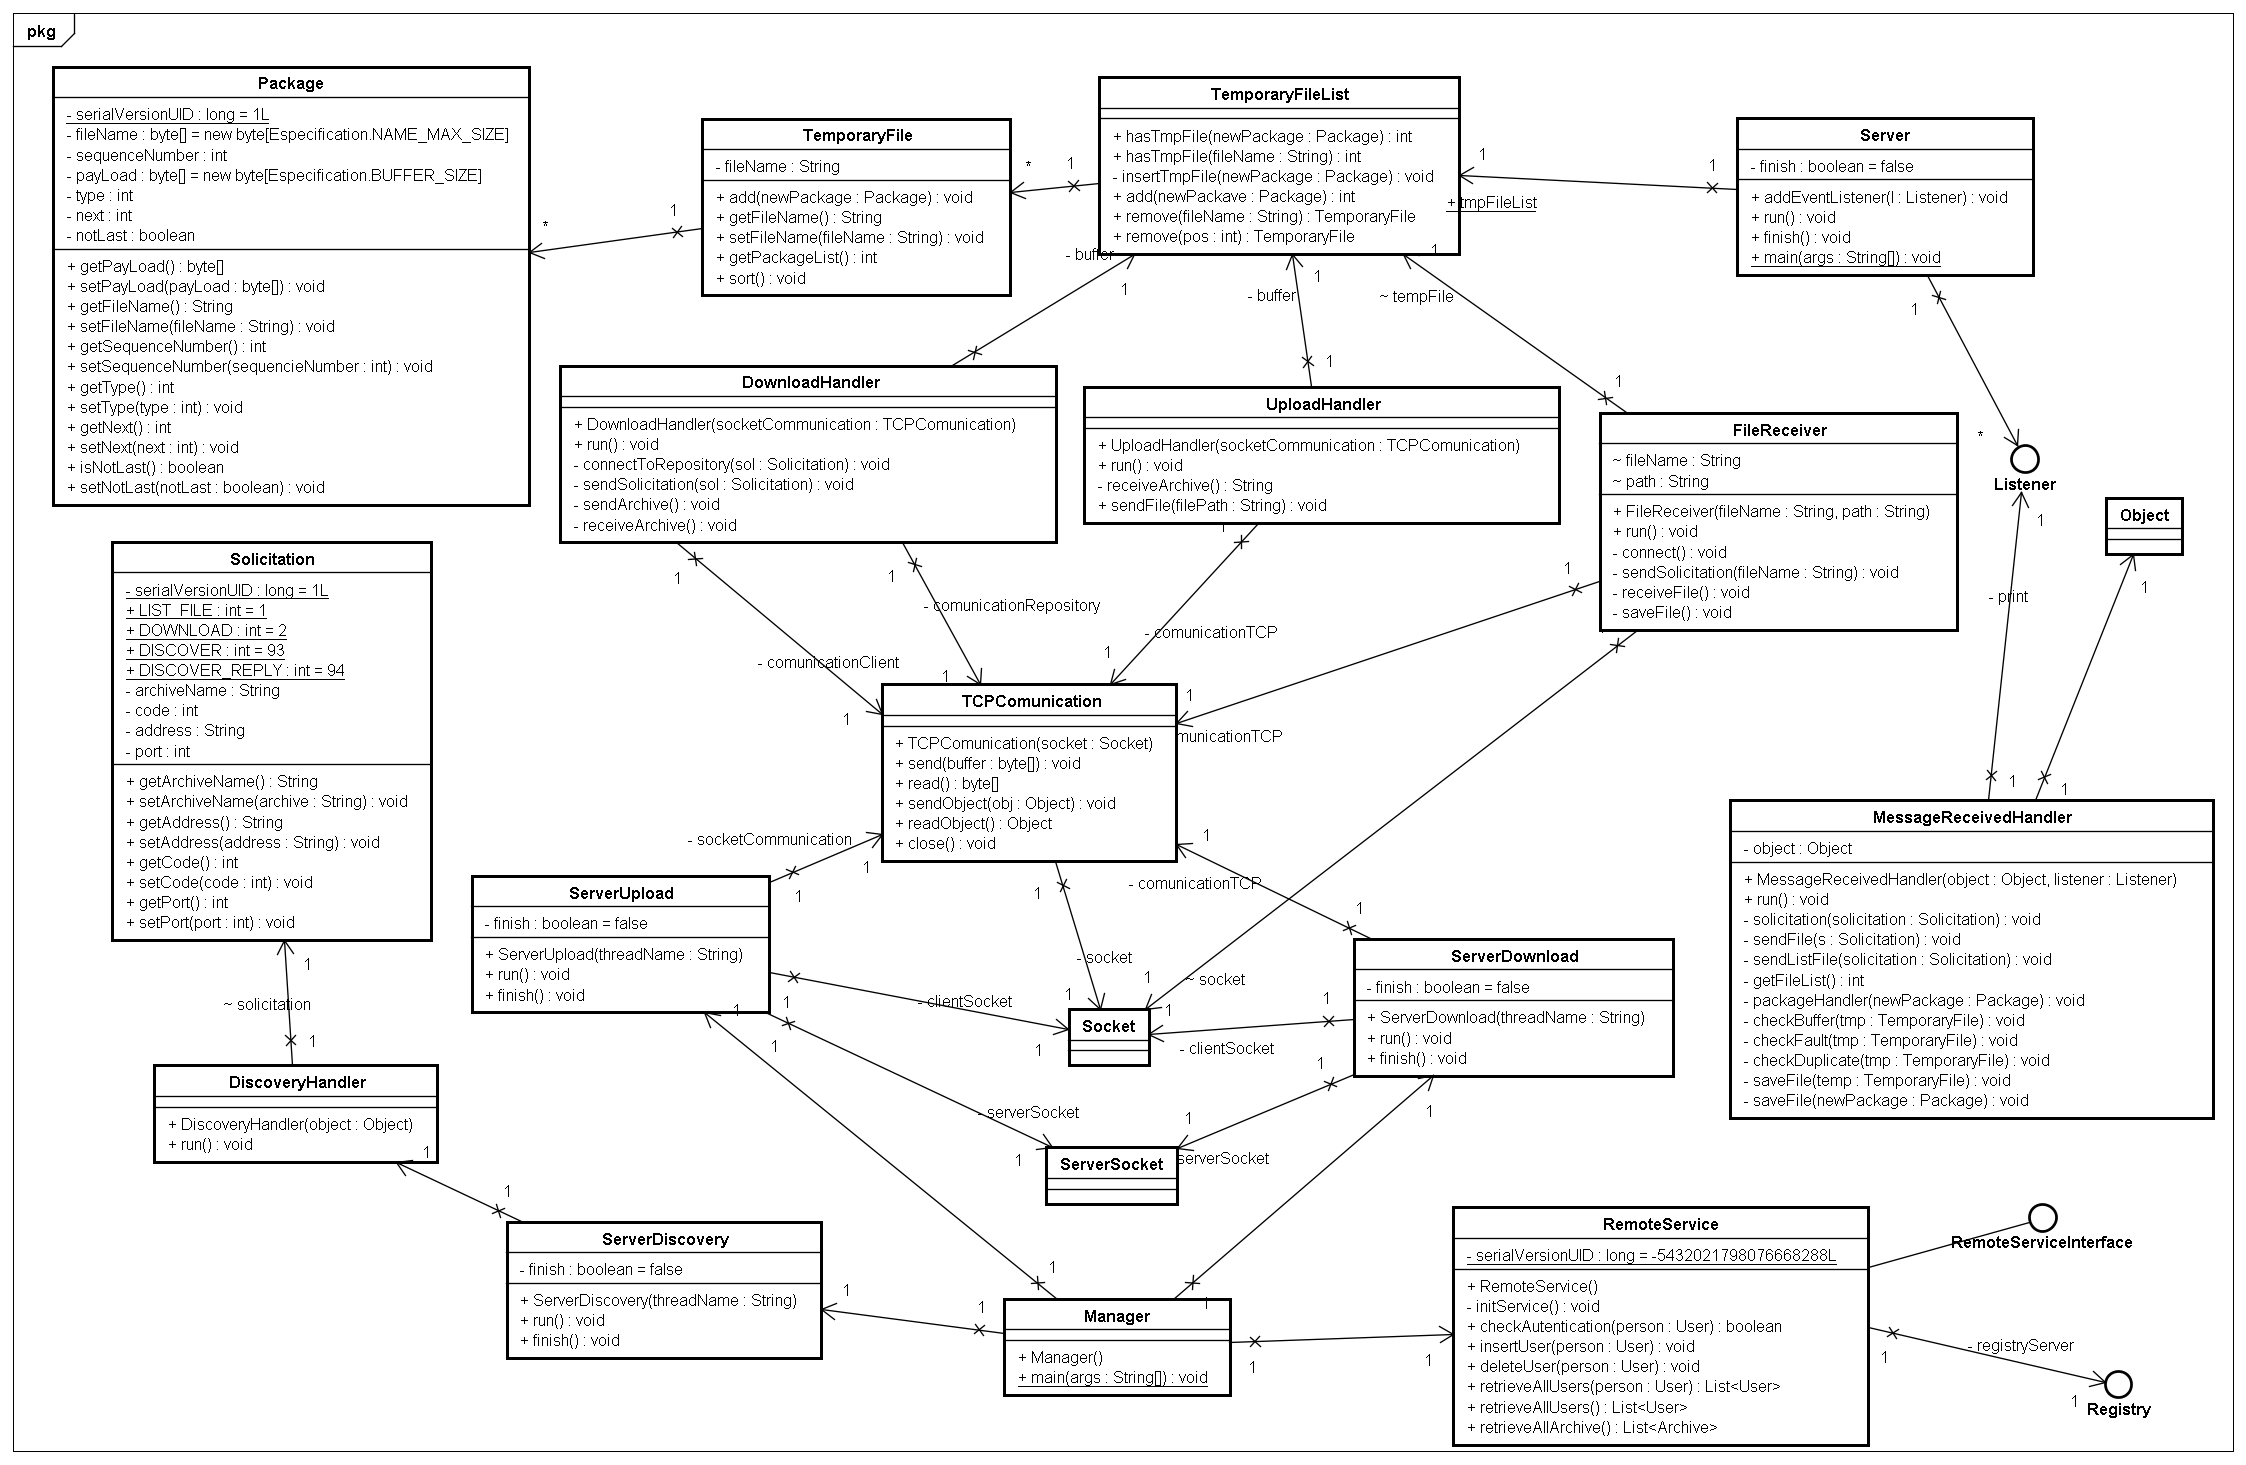
\includegraphics[scale=0.3]{figuras/diagrama-classes.png}
		\caption{Diagrama de Classes do SDA.}
 		\label{figura5}
	\end{figure}
	
\chapter{Como utilizar o SDA}

	\indent Para utilizar o sistema SDA, primeiramente se faz necess�rio inicializar os arquivos SDA-server.jar e SDA-manager.jar respectivamente no computador sevidor. Ao serem inicializadas, aparecer�o as interfaces a seguir (Figura \ref{figura1}).
	
	\begin{figure}[!htb]
	\begin{minipage}[b]{0.40\linewidth}
	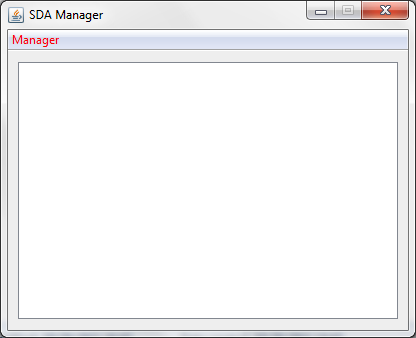
\includegraphics[width=\linewidth]{figuras/manager.png}
	\end{minipage} \hfill
	\begin{minipage}[b]{0.40\linewidth}
	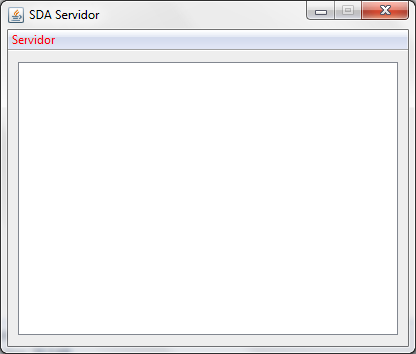
\includegraphics[width=\linewidth]{figuras/servidor.png}
	\end{minipage}
	\caption{Telas Manager e Servidor} \label{figura1}
	\end{figure}
	
	Nestas telas aparecer�o todas informa��es que trafegar�o pelo SDA, tais como, clientes conectados, arquivos recebidos, arquivos enviados, pacotes em  que foram divididos tais arquivos, etc. 
	
 	No computador cliente dever� ser inicializado o arquivo SDA-cllient.jar, onde primeiramente aparecer� uma tela para que seja informado o IP do computador servidor, como a mostrada na figura \ref{figura2}.
 	\begin{figure}[!htb]
		\centering
		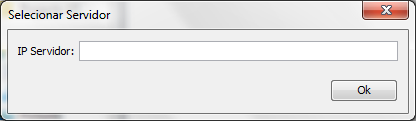
\includegraphics[scale=0.35]{figuras/antes-cliente.png}
		\caption{Configura��o IP servidor.}
 		\label{figura2}
	\end{figure}

	Posteriormente aparecer� uma tela para autentica��o do cliente, esta tela � mostrada na figura \ref{figura3}.
	
	\begin{figure}[!htb]
		\centering
		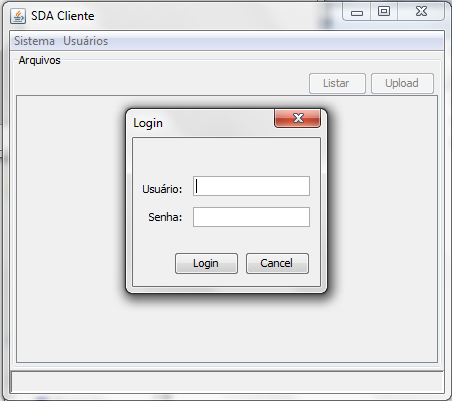
\includegraphics[scale=0.35]{figuras/sda-cliente-login.png}
		\caption{Autentica��o do cliente.}
 		\label{figura3}
	\end{figure}
	
	Por fim aparecer� a tela principal do cliente. Nesta tela, o cliente tem a op��o de listar todos arquivos presentes no servidor, al�m de fazer gravar arquivos no servidor. Esta tela � mostrada na figura \ref{figura4}.
	
	\begin{figure}[!htb]
		\centering
		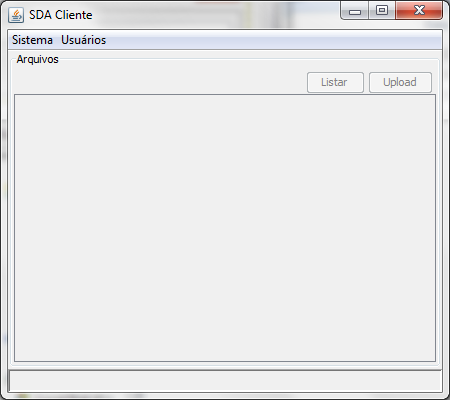
\includegraphics[scale=0.35]{figuras/cliente.png}
		\caption{Tela principal cliente.}
 		\label{figura4}
	\end{figure}
	
\chapter{Datas e Horas Trabalhadas}

	\indent Para o desenvolvimento deste aplicativo foram necess�rias algumas horas dedicadas durante v�rios dias. Abaixo temos a listagem dos dias e a quantidade de horas trabalhadas:
	
	\begin{itemize}
		\item 15/08/2011 - 1 hora trabalhada;
		\item 23/08/2011 - 2 horas trabalhadas;
		\item 07/09/2011 - 2 horas trabalhadas;
		\item 13/09/2011 - 1 hora trabalhada;
		\item 22/09/2011 - 2 horas trabalhadas;
		\item 02/10/2011 - 2 horas trabalhadas;
		\item 08/10/2011 - 2 horas trabalhadas;
		\item 10/10/2011 - 2 horas trabalhadas;
		\item 11/10/2011 - 2 horas trabalhadas;
		\item 17/10/2011 - 3 horas trabalhadas;
		\item 18/10/2011 - 3 horas trabalhadas;
		\item 19/10/2011 - 3 horas trabalhadas;
		\item 20/10/2011 - 3 horas trabalhadas;
	\end{itemize} 
	
	No total foram necess�rias 30 horas de trabalho para o desenvolvimento desta aplica��o.
	
{\color{white}\cite{coulourissistemas}}
		
		



%-----------------------------------------------------------------
%BIBLIOGRAFIA
%-----------------------------------------------------------------
\bibliography{bibliografia}
\bibliographystyle{abnt-alf}

%-----------------------------------------------------------------
\newpage
\end{espacoumemeio}
\end{document}
%-----------------------------------------------------------------